
In a second set of \Q-learning experiments, we examined the impact of
endowing agents with \mydef{social preferences}. That is, their
rewards no longer depend solely on their own successes and
failures---they depend on those of other agents in the environment as
well.

To make this idea more precise, we separate \mydef{objective} and
\mydef{subjective} reward. Objective reward is the usual reward
signal provided to the agent from the environment, and by which
behavior is judged. Standard reinforcement-learning agents, such as a
\Q-learning agent, seek to optimize their own objective reward
signal---we call this preference the ``selfish'' preference because
these agents are only concerned with their own outcomes.

In some environments, however, it useful to distinguish this objective
reward from subjective reward---the quantity the agent \emph{believes}
it should be optimizing. Previous work has shown that optimizing
subjective reward can sometimes lead agents to be more effective in
their acquisition of objective reward~\cite{singh2009rewards}.  (Indeed, we
reach this same conclusion in our experiments.)

Considering the four different outcomes in these games---{\bf GG},
{\bf GN}, {\bf NG}, {\bf NN}---there are 75 different possible
preference orderings (allowing for ties). The selfish ordering that
ignores the opponent's outcome is one of these:
{\bf GG} $\sim$ {\bf GN} $\succ$ {\bf NG} $\sim$ {\bf NN}.
%Regardless of the opponent's outcome, a selfish agent only prefers that it gets to its goal. 
Nine of the 75 orderings are consistent with the selfish ordering,
strictly preferring {\bf Gx} to {\bf Nx} for all {\bf x}.

Of particular interest is the \mydef{fair} preference, which we define
as the objective reward of the agent minus 25\% of the difference
between its own and the opponent's objective rewards:
$r_{s} = r_{a} - 0.25 \left| r_{a} - r_{o} \right|,$ where $r_{s}$
is the agent's subjective reward, $r_{a}$ is the agent's objective
reward, and $r_{o}$ is the opponent's objective reward.\footnote{Other
percentages would achieve the same result.}  By incorporating this
fairness term into the agent's subjective reward, it strictly prefers
the following ordering:
{\bf GG} $\succ$ \mbox{\bf GN} $\succ$ \mbox {\bf NN} $\succ$ {\bf NG}.
That is, the agent prefers making it to its goal as opposed to not,
but it additionally prefers that the opponent only get to its goal if
the agent itself does as well. To say it another way, a fair agent
wants its opponent to win with it or lose with it.

%%JLA: I was tempted to write here that Tit-for-Tat has a flavor of ``fairness'' preference, but I'm too tired to think through this properly.

%\begin{wrapfigure}{l}{0.4\textwidth}

%\end{wrapfigure}

Figure~\ref{f:selfplay} shows the result of the selfish and fair
agents playing against others of the same type in each of our test
grid games.  Of the nine orderings, only three (all variations of the
fair preference ordering) achieve consistent cooperation in self play
across all five grid games.  Consequently, fair agents obtain higher
total (objective) rewards than others.  
%
We also ran all nine preference orderings against one another.  The
average scores (across both players) in games involving a fair agent
tend to be higher than the average scores in games not involving a
fair agent.

\comment{
\begin{figure*}
\centering
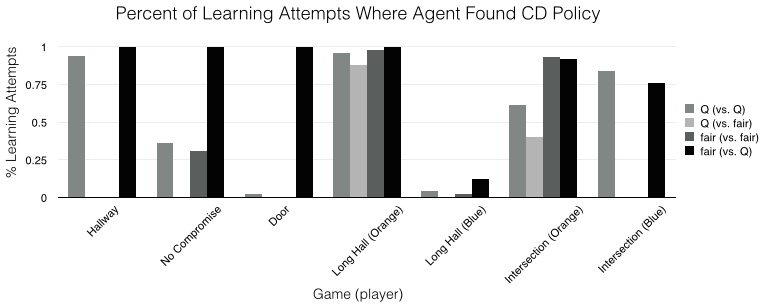
\includegraphics[width=1.5\columnwidth]{figures/ConvCD.png}
\caption{The percentage of learning attempts where the agent's final policy was CD by game and learning opponent.}
\label{f:convCD}
\end{figure*}

In Figure~\ref{f:convCD}, we show results on the classification of
policies found by the agents when learning against opponents of
different preference types. These results show that the fair agent
(\Q-learning with preferences in Equation~\ref{e:fair}) finds a CD
policy as frequently as or more frequently than normal
selfish \Q-learning when trained against another \Q-learning agent or
when trained against a fair agent. The exception is Blue in
Intersection. Across all five games and all agent positions, the
selfish agent finds a CD policy in 50.9\% attempts when learning
against selfish and in 12.8\% of attempts against the fair agent. The
fair agent's performance in these cases is 88\% and 25.5\%,
respectively. These results suggest that \Q-learners with fair
preferences may find CD policies more often, especially when they
learn against a selfish player. Whether this is general for a broader
set of grids is an important question for future work.
}

We also analyzed the types of strategies learned by fair and
selfish \Q-learners after multiple simulations of various
configurations. Interestingly, we found that \Q-learners with fair
preferences tend to find CD strategies more often, especially when
paired with selfish agents.

In summary, \Q-learners naturally learn to cooperate in the grid games
studied, discovering equilibria comprised of CD strategies when they
exist.  Cooperation can be induced in other games by manipulating
the \Q-learners' subjective rewards to incorporate the success of others.

In the next section, we describe analogous experiments conducted with
humans playing grid games.  In those experiments as well, we were able
to manipulate the rewards to favor fairness, and doing so induced more
cooperation than otherwise.

\comment{
Given the option of who to play with, agents do best when playing
against the fair preference ordering. We also analyzed which
preference ordering is the preferred one to adopt. It turns out that
the preference ordering {\bf GN} $\succ$ {\bf GG} $\succ$ {\bf NG}
$\sim$ {\bf NN} is an evolutionary stable strategy---it outperforms
competitors in a population and can maintain its dominance against
invaders. It adopts a much more aggressive stance that the fair
preference ordering in that it prefers winning alone to sharing the
top spot. Thus, it has a tendency to find strategies that drives its
opponents' scores down.
}

